\cleardoublepage
\newrefsection
\chapter{外文翻译}

\section{摘要}

在这篇综述中,我们将讨论了联合反演和约束反演方法的基本原理,并展示了这些方法在文献中应用的几个有启发性的例子。从术语联合反演和约束反演的一些基本定义开始,我使用一个简单的三层模型作为教程,演示了具有不同耦合方法的联合反演的一般属性。特别地,我调查了不同地球物理方法的组合在多大程度上可以限制可接受的模型集,以及在什么情况下结果可能有偏差。关于如何识别这种有偏见的结果以及如何解释负面结果的一些想法总结了教程部分。第二部分的案例研究被选中以突出具体问题,例如选择适当的参数关系来耦合地震和电磁数据,并展示最常用的方法,例如交叉梯度约束和直接参数耦合。在整个讨论过程中,我试图确定未来工作的主题。总的来说,将电磁数据与其他观测相结合似乎已经趋于成熟,并开始从基本的概念验证研究转向回答有关地下结构的问题。通过适用于不同地质情况的多种耦合方法,综合方法可以应用于所有尺度,并有可能为重要的地质问题提供新的答案。

\section{简介}

地球物理观测反演是研究地球地下和了解我们赖以生存的星球的结构和组成的主要工具之一。钻孔通常使我们能够接触到5公里深处的材料,在特殊情况下可达10公里(Huenges等,1997),但只能在特定位置取样。在某些地方,例如金伯利岩管,地质过程将物质从深处输送到地表,并为我们提供来自下地壳和地幔的样本(例如,Griffin等,2009)。然而,我们的大部分知识来自将假设模型计算出的数值模拟的输出与地球表面或附近的地球物理观测结果进行比较。在某些情况下,这些模型是通过正演建模通过反复试验生成的(Leibeckeretal.,2002;Gatzemeier and Moorkamp,2005;Heise等,2008)。如果这个过程执行得好,我们可以测试关于所调查区域物理结构的不同假设,并深入了解数据对不同结构的敏感性。然而,正演建模通常需要大量试验,因此是一项乏味的任务。此外,模型通常是对地质结构的强烈概括,先入为主的想法可能会影响在此过程中考虑的模型类型。
由于这些原因以及过去几年计算能力的显着提高,如今大多数地球物理模型都是通过正式的反演程序构建的。在这里,我们在数学上定义可接受模型的标准,通常是最终模型预测的数据符合最小二乘意义上的观察结果(例如,Wheelock等,2015),并使用自动算法找到一个或一组满足这些标准的模型。鉴于反演不仅在地球物理学中的重要性,存在大量不同的算法来完成这项任务(Nocedal2006)。Snieder和Trampert(1999)、Tarantola(2004)、Menke(2012)、Mosegaard和Hansen(2016)以及大地电磁法(MT)和受控源的特殊情况对地球物理背景下的反演方法进行了很好的介绍Avdeev(2005),Abubakar等的电磁学(CSEM)。(2009)、Siripunvaraporn(2012)以及Rodi和Mackie(2012)。
尽管有高度精确的算法和深入的研究,地球物理数据的反演实际上总是病态的,即相似的数据可能导致截然不同的模型(例如,Backus和Gilbert1967)和非唯一的,即无限数量的模型可以解释数据相同程度的不确定性(例如,Munooz和Rath,2006)。这是因为我们只能在地表或地表附近进行测量,并且与地质变化的尺度长度相比,站点之间的距离很大。此外,我们的测量是带限的并且受到噪声的污染(Parker1980,1983)。这导致在解释数据时需要考虑的逆向模型中的歧义。然而,这些歧义的本质是特定于方法的。例如,大地电磁法可以很好地解析电阻层的厚度,但不能解析电阻率,而直流电阻率对其电阻很敏感,即电阻率‑厚度乘积(Vozoff和Jupp,1975)。如果我们能够利用这些互补的敏感性,与仅使用单一方法相比,我们有望更好地恢复地球内部结构的形状和特性。
这是联合合作反演的核心思想:我们将来自两种或多种不同类型的地球物理数据集的信息组合在一个反演算法中,目的是改进所得模型。本综述的目的是解释和说明联合反演的不同方法,特别强调电磁方法。我将给出联合反演的工作定义,并将其与其他合并不同数据集的方法进行简要比较和对比。然后我将展示一些精选的使用联合反演方法时展示优势和潜在缺陷的示例。最后,我将尝试总结我们目前所处的位置以及未来的途径。与Haber和HoltzmanGazit(2013)最近对该主题的评论相比,我将重点关注概念和应用,而不是数学细节。

\section{关于联合反演的简介}

出于回顾的目的,我将使用术语联合反演来表示在单个计算算法中使用单个目标函数对不同类型的数据进行反演并且在整个反演过程中同时调整所有模型参数的所有方法(Moorkamp等.2016b).特别感兴趣的是联合反演方法,它结合了不同的物理特性,例如电导率和地震速度,因为这些提供了巨大的潜在好处,但也带来了特殊的问题。相比之下,合作反演包括仅对单个数据集进行反演并将另一个反演的结果用作参考的方法(例如,Paasche和Tronicke,2007)。在这篇评论中,我不会讨论反演后积分背后的理论,其中以定量方式检查从独立反演中检索到的模型的关系(例如,Bedrosian等,2007),并且可以在Paasche中找到很好的概述(2016)、Bedrosian(2007)和Hansen等。(2016)。

正如联合反演的定义所暗示的那样,首要和关键步骤之一是定义优化算法将最小化的目标函数。在最一般的形式中,这个目标函数可以写成以下形式:

\begin{equation}
    \Phi_{joint}(\mathbf{m}) = \Phi_{data}(\mathbf{m}) +\lambda \Phi_{reg}(\mathbf{m})+\mu \Phi_{coupling}(\mathbf{m})
\end{equation}

这里$\Phi_{data}(\mathbf{m})$和$\Phi_{reg}(\mathbf{m})$在数学上定义了模型参数的不同子集之间的关系。注意在这种通用表示法中,模型向量$\mathbf{m}$可能包含与非 常不同的数量相关联的元素。例如,当联合反演分层地球结构的大地电磁和地震走时数据时,前N 个模型参数 可以是反演中使用的N个层的电阻率,第二个N个模型参数指定相同层的地震速度。耦合项然后在这两组模 型参数之间建立关系,该关系指定我们要执行哪种联合反演。

对于协同反演,数学公式看起来是一样的。同样,我们有一个数据误差项、一个正则化项和一个耦合项,只是 现在数据误差和正则化仅针对电阻率进行计算,例如,地震速度模型被认为是固定的并且仅用于耦合项以最大化模型之间的相似性。下图显示了两种方法之间的差异,作为反演的流程图。

我现在将讨论一系列非常简单的实验,以说明联合和协作反演的一些基本性质以及常见的耦合方法及其性 质。所有实验的基础是从一个简单的一维三层模型计算的数据(图2)。为了进一步简化讨论并提供帮助可视化,我也假设知道最上层和最下层的物理特性(电阻率和地震速度)和厚度,并且只寻求中间 层的厚度和物理特性。因此,逆向问题简化为为每个地球物理数据集寻找两个模型参数,例如MT 的第二层电阻率和厚度,并且很容易将可能解的范围绘制为简单的散点图。

\begin{figure}
    \centering
    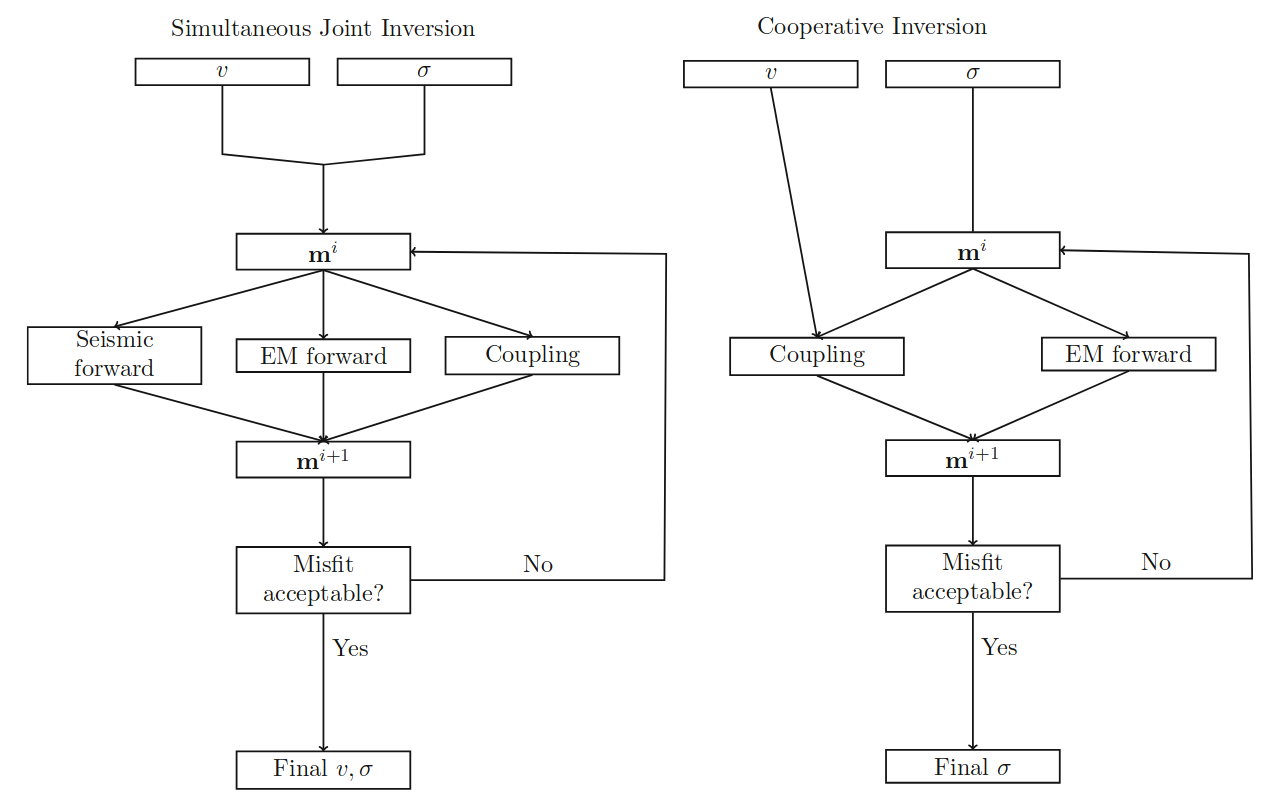
\includegraphics[width=0.9\textwidth]{trans/trans_1.png}
    \caption[]{联合反演算法(左)和约束或协作反演算法(右)的简化流程图(Moorkamp等, 2016 b)。两种方法之间的主要区 别在于,对于协同反演,进入耦合约束的一个量(此处地震速度 v)在整个反演过程中不会发生变化,而所有量都在联合反演中进行调整}
\end{figure}

\begin{figure}
    \centering
    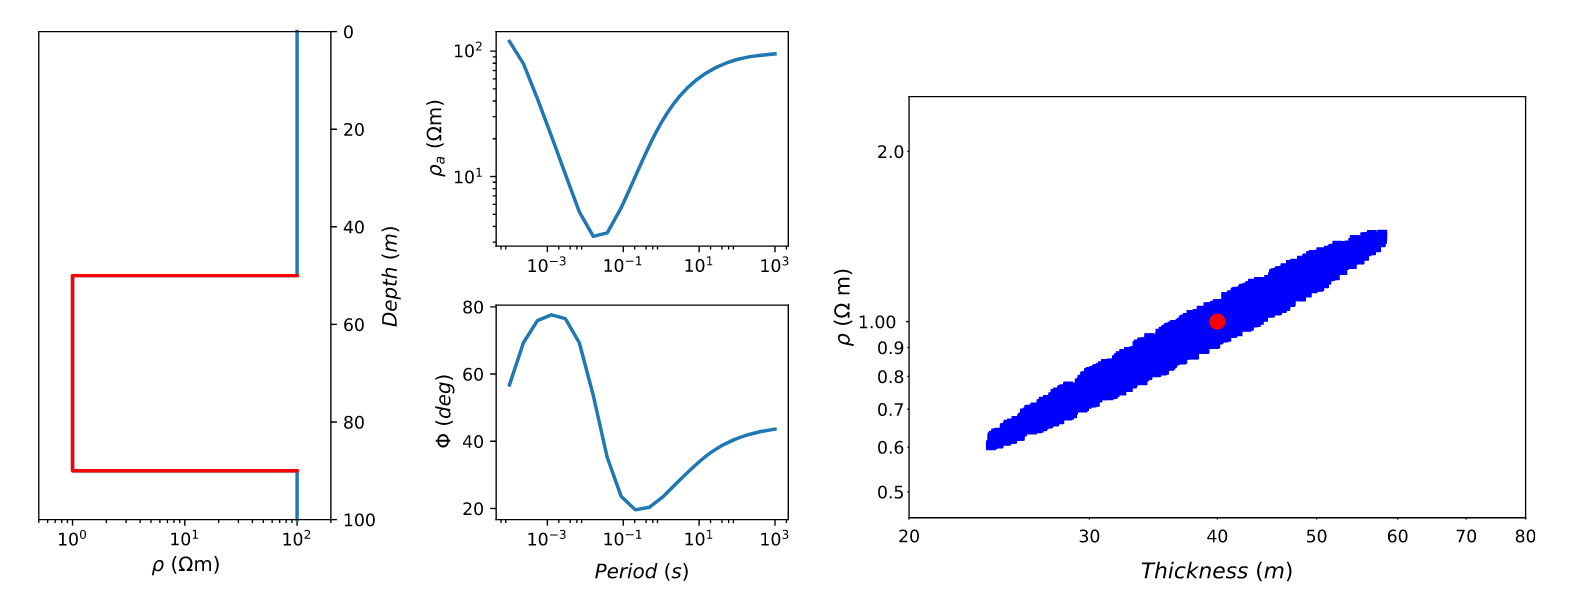
\includegraphics[width=0.9\textwidth]{trans/trans_2.png}
    \caption[]{简单的大地电磁测试模型(左),该模型的正向响应(中)和仅反演 MT 数据时可接受的反演模型空间(右)。在整个教程 中,仅假设最上层和最下层是已知的,只求中间层(标记为红色)的厚度和电阻率}
\end{figure}

图2显示了真实模型(左),其中我们要反演的层标记为红色。从模型(中间的图)预测的大地电磁数 据显示典型的三层响应。为了说明可行的解决方案,我简单地生成了大量试验电阻率和厚度的随机组合,计算出与真实响应的误差,并保留拟合数据的实部和虚部均在 2\%以内的参数组合。生成的可行解在图2中显示为蓝点,真实值显示为红色。这个简单的实验证明了众所周知的无法恢复薄导电层的电阻率和厚度,而不是层电导,即电导率与厚度乘积受到很好的约束。该特征在反演问题的解集中清晰可见。查看反演问题的解,该层可以具有20 m和60 m之间的任何厚度,同时也有合适的电阻率。

\begin{figure}[H]
    \centering
    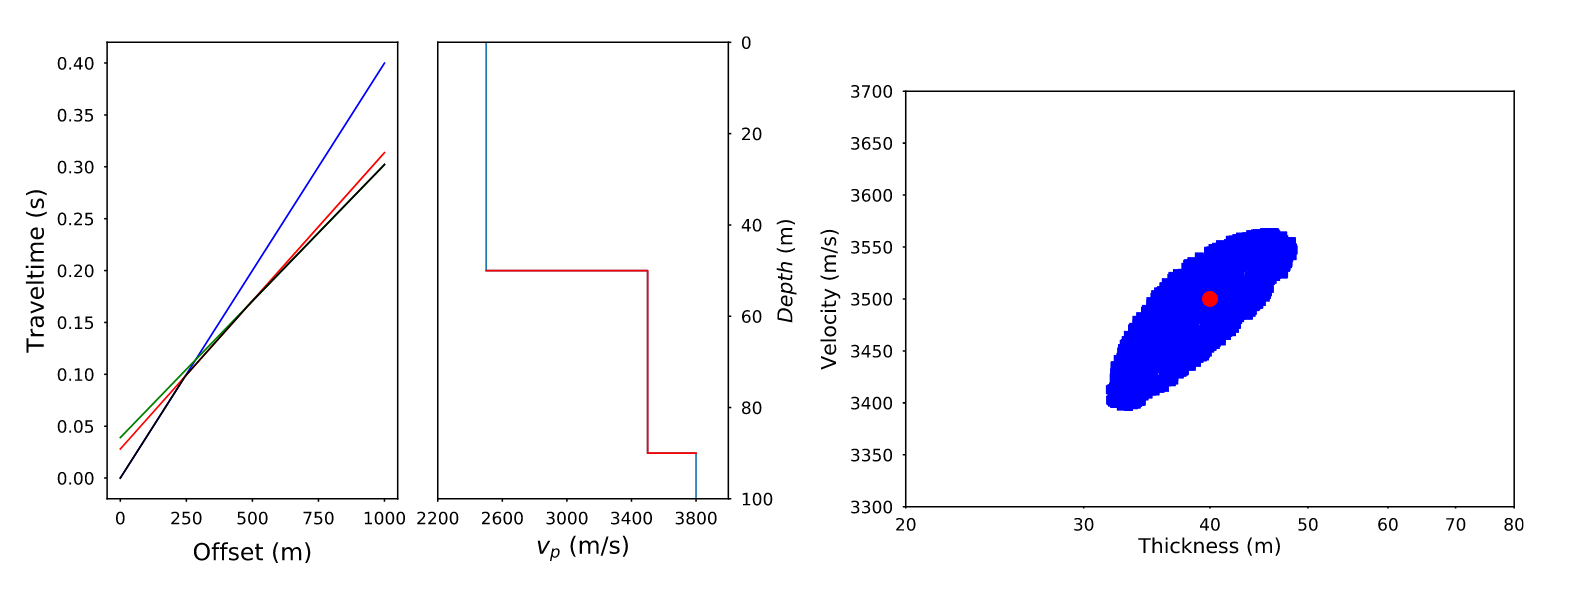
\includegraphics[width=0.9\textwidth]{trans/trans_3.png}
    \caption[]{单独反演走时时的地震数据(左)、真实模型(中)和一组可接受的速度与厚度的组合(右)。对于图3.2中的   MT  情况,只有 中间层(标记为红色)的属性被认为是未知的}
\end{figure}

如果我们在同一位置进行地震折射实验并仅从这些测量中确定一组允许的解决方案,我们将得到图3 所示的 结果。在这种情况下,地震折射数据也显示出模糊性以及速度和速度的范围解释假设误差内观察结果的厚度值。 然而,与大地电磁方法相比,可能的厚度值范围更窄,在30到 45m 之间。联合反演的核心思想是在两种方法感知相同结构的假设下,找到解释两个数据集的模型将导致更好地恢复这些 结构。现在,我将讨论最常用的假设,并通过这些简单的示例演示如何使用它们、可以期待什么样的改进以及存在 哪些缺陷。


\subsection{结构耦合}

关于不同地球物理方法之间的关系,我们可以做出的最普遍的假设之一是它们感知地球内部的相同地质结构,特 别是它们的边界。因此,如果有任何速度或电阻率异常,它们应该发生在同一位置。因此,结构联合反演方法不规定 不同物理参数之间的任何直接相关性,而是使用这些参数变化之间的空间关系来耦合不同的方法(Haber 和 Oldenburg,1997; Gallardo 和 Meju,2003)。我将在下面的案例研究中讨论联合反演中常用的不同结构 关系的一些例子。对于分层地球,一个简单的结构关系是假设所有方法的反演中的层边界都处于相同深度(例如, Manglik 和Verma,1998; Moorkamp等,2007;泽瓦洛斯等。 2009; Moorkamp 等。2010; Roux 等,2011; Juhojuntti 和Kamm,2015)。图4显示了假设边界重合时我们的简单示例的两个数据集的可接受模型范围。

\begin{figure}
    \centering
    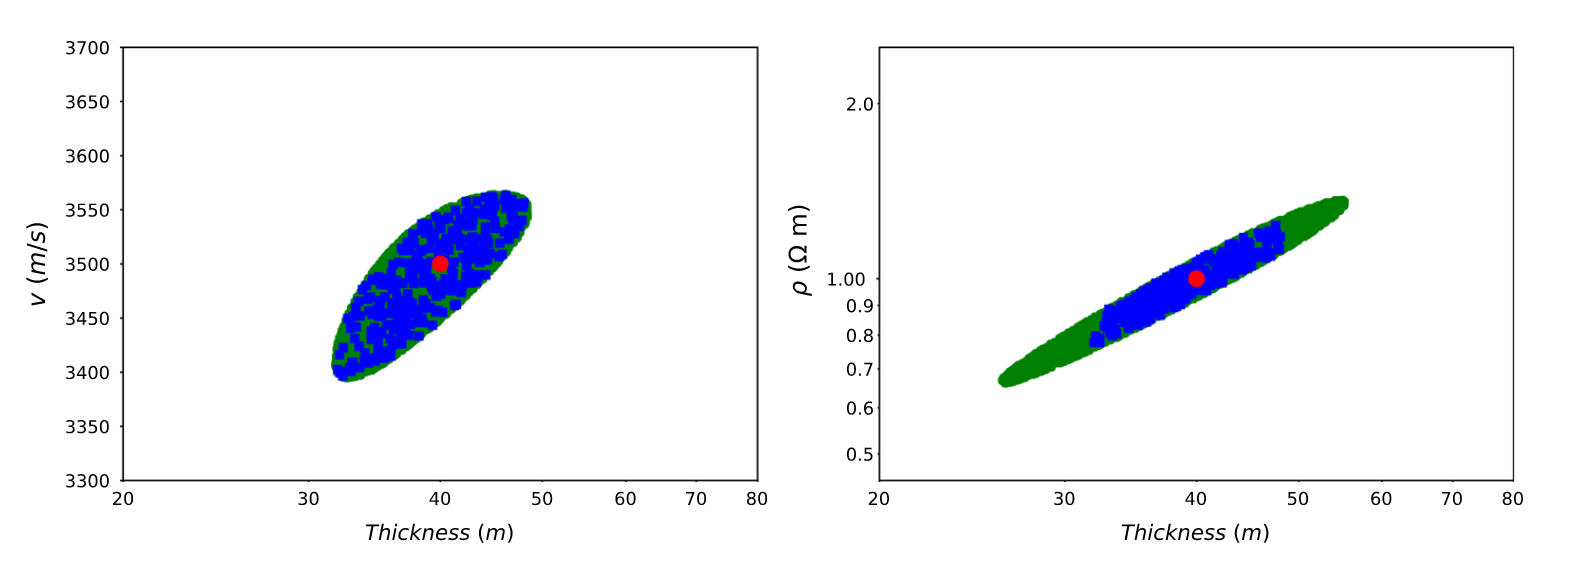
\includegraphics[width=0.9\textwidth]{trans/trans_4.png}
    \caption{一组可接受的速度-厚度(左)和电阻率-厚度(右)组合,用于单独反演和联合反演,具有基于重合层厚度的结构约束。单 独反演的可接受模型标记为绿色,而联合反演模型标记为蓝色}

\end{figure}

由于没有采用电阻率和速度之间的关系,因此这种方法主要限制了允许的层厚度范围。鉴于大地电磁数据的这个范围较大,允许的电阻率模型的范围减小,而可接受的地震模型的范围与单独的分析相同。总的来说,结构耦 合实现了联合反演的主要目标,以减少可接受模型的范围,即使在这种情况下仅针对一个参数子集。显然,对于更为实际的反演,即假设地球是分层的,情况也会更加复杂。当同时反演所有三层的属性时,不同层的厚度和物理参 数之间存在显着的相互作用。例如,大地电磁数据对顶层厚度具有合理的敏感性,该信息将有助于约束地震模型, 进而有助于约束第二层的厚度。因此,在现实世界的联合反演中,并不总是那么清楚哪种方法主导分辨率属性,并 且在许多情况下,不同的方法驱动模型域不同部分的反演(Jegen 等,2009 ; Heincke 等,2009 )。 2014; Demirci 等, 2017 )。我将在应用部分讨论其中的一些问题;现在我将继续这个简单的 例子,因为它提取了联合反演的许多重要方面。

进一步考虑层厚度的分辨率如何从速度模型转移到电阻率模型,以及它如何影响图4中可接受模型的范围,同 样清楚的是,我们将找到适合两个数据集的模型,即使厚度真实速度模型中的层数不同于真实电阻率模型。60 m的厚度在大地电磁数据的可接受范围内,因此,将层厚度为 40 m的电导率模型与地震厚度为60 m的组合将 产生一个联合模型,该模型在假设的范围内拟合两个数据集噪音水平。在最极端的情况下,真实地震模型的层厚 可能超出大地电磁数据的允许范围,但考虑到地震结果的不确定性,这两个区域重叠,我们找到了一个适合两个数据集的联合模型到可接受的水平,但两种方法都处于极端不确定的状态。

在这个非常简单的例子中,进行协同反演最直接的方法是选择一个适合地震数据的模型并将其用作参考MT的模型。在最受约束的情况下,我们可以将该模型的层厚度作为真实层厚度的估计值,并且只搜索电阻率。结果 是一组非常有限的可接受模型。然而,如果估计厚度与真实厚度不同,则真实模型将不包括在可接受的模型集中并 且估计的电阻率将有偏差。一种更接近当前实践的方法(Kalscheuer  等,   2015)是在目标函数中包 含一项,要求层的厚度尽可能接近地震估计值。

图5显示了可接受的模型,这些模型与   50   m   的估计层厚度一致,误差在   10\%  以内。与指定固定层厚相比,可接受 模型的范围有所增加,但仍小于结构耦合联合反演。根据厚度估计和我们在估计中指定的不确定性,真实模型将 是否包含在可接受的模型中。在我们有关于可接受地震模型范围的全部信息的情况下,例如,从概率反演方法,结 果将与联合反演结果相同。然而,如果我们只有一个模型和模型不确定性的临时估计,那么结果在很大程度上取决于这两者与真实模型的关 系。 MT的模型。在最受约束的情况下,我们可以将该模型的层厚度作为真实层厚度的估计值,并且只搜索电阻率。结果 是一组非常有限的可接受模型。然而,如果估计厚度与真实厚度不同,则真实模型将不包括在可接受的模型集中并 且估计的电阻率将有偏差。一种更接近当前实践的方法(例如,Kalscheuer  等人,   2015   年)是在目标函数中包 含一项,要求层的厚度尽可能接近地震估计值。 起初,看到合作或约束反演比完全联合反演更能限制可接受模型集可能会令人惊讶。虽然解释相对简单:由于 无法对参考模型进行调整,除非我们考虑完整的后验模型协方差,否则地震数据的不确定性已从等式中剔除。因 此,必须特别小心地检查作为此类约束反演结果的模型,并且可以将其视为假设检验的特殊情况,如下所述,即我 们已经证明存在类似于地震参考模型并适合大地电磁法的模型数据。

\subsection{基于参数关系耦合}

通过结构耦合方法不对不同地球物理方法之间的关系做出强假设,因此具有广泛的适用性。正如示例所示,与单独的反 演相比,这样做的结果可以适度提高分辨率。如果我们在反演中利用更多关于地球的信息,我们可能会显着改善 我们的结果。这通常适用于所有逆向方法,额外的先验信息限制了可接受模型的空间,但存在使解决方案产生偏差 的风险(Tarantola   2004;   Mosegaard  和   Hansen  2016)。
